\chapter{Einleitung}

In diesem Kapitel gebe ich eine Einführung in die Thematik der vorliegenden
Bachelorarbeit. Ich erläutere und motiviere die Zielsetzung des Projektes und
beschreibe den Umfang und Aufbau meiner Arbeit.

\section{Motivation}

Der Computer ist allgegenwärtig, und zu ihm gehört seit jeher die Tastatur.
Ursprünglich von der Schreibmaschine inspiriert, wurde sie zum primären
Eingabegerät für PCs und ist nun von keinem Schreibtisch mehr wegzudenken. Auch
den Übergang zu anderen Geräten, etwa Smartphones und Tablets, hat die Tastatur
mitgemacht -- teils in Form echter Tasten auf dem Gerät, teils virtualisiert
auf einem Touchscreen.

Es gibt viele Gründe für die weitreichende Verbreitung von Tastaturen. Zunächst
ist ihr Prinzip sehr einfach, somit ist ihre Bedienung leicht zu erlernen, und
mit etwas Übung wird ein Benutzer auch schnell effizient in ihrer Verwendung.
Außerdem ist die Herstellung einer Tastatur aufgrund der technischen
Einfachheit günstig. Es kommt hinzu, dass sie sehr präzise arbeitet -- drückt
man die richtige Taste, kann der Computer dies mühelos interpretieren, es gibt
keinen Raum für Fehler.

Allerdings haben Tastaturen viele Nachteile. Allen voran ist die Problematik
der Ergonomie zu nennen. Viele Bürokrankheiten haben entweder mit der
Überlastung des Hand\-ap\-pa\-ra\-tes zu tun oder werden durch die zwanghafte
Sitz\-hal\-tung verursacht, die unter anderem durch die Verwendung einer
Tastatur vorgeschrieben wird~\citep{disorders}. Auch sind Menschen mit
eingeschränkten motorischen Fähigkeiten, etwa aufgrund von Krankheiten oder
fehlender Finger, nicht in der Lage, mit vergleichbarer Effizienz die Tastatur
zu benutzen.

Zudem sind Tastaturen relativ groß und somit nur eingeschränkt portabel. Auf
den immer kleiner werdenen mobilen Geräten wird die Erforderlichkeit einer
Tastatur immer mehr zum limitierenden Faktor. Auf einer ,,Smartwatch'' zum
Beispiel gibt es in der Regel aufgrund der Größe keine eigene Tastaturfunktion,
man muss diese mit einem Mobiltelefon verbinden.

Außerdem sind Tastaturen nicht flexibel für unterschiedliche Anwendungsfelder
einsetzbar. Ein Beispiel ist die Grafikbearbeitung, bei welcher der Benutzer
stufenlose Werte wie Pinselgröße oder Farbe anpasst. Die Tastatur mit ihren
binären Tasten liefert hierfür keine zufriedenstellende Möglichkeit.  Auch die
Verwendung von Tastenkürzeln, bei der mehrere Tasten in Kombination gedrückt
werden, um eine andere Funktion als Texteingabe zu bewirken, ist nicht
benutzerfreundlich und vielen Benutzern
unbekannt~\citep{lane-keyboard-shortcuts}.

\section{Vision} \seclabel{vision}

In diesem Projekt versuchen wir\footnote{Ich verwende in dieser Arbeit die
erste Person Singular (,,ich''), um den Inhalt meiner Arbeit wiederzugeben, und
die erste Person Plural (,,wir''), wenn ich mich auf das gesamte Projekt
beziehe.}, eine Alternative zur klassischen Tastatur zu entwickeln. Wir möchten
ein System entwerfen, welches Text- und Zeicheneingabe, aber auch sonstige
Interaktion mit einem digitalen Gerät ermöglicht, und dabei möglichst wenige
der oben genannten Nachteile klassischer Tastaturen mit sich bringt. Das Tippen
soll dabei komfortabler und flexibler werden.

Dazu möchten wir uns im ersten Schritt nicht zu weit von der gelernten
Texteingabemethode entfernen. Die Bewegungen der Hand, die ein geübter
Tastaturbenutzer im Muskelgedächtnis gespeichert hat und somit mühelos
durchführen kann, möchten wir aufzeichnen und zu Tastendrücken konvertieren,
ohne dass dafür die Verwendung einer herkömmlichen Tastatur nötig wäre. Dafür
soll unser System in der Lage sein, die Bewegungen der Finger und der ganzen
Hand zu messen und mithilfe maschinellen Lernens aus diesen die gedrückten
Tasten abzuleiten.

\section{Zielsetzung und Umfang}

Da sich das Projekt im Umfang an 2 Bachelorarbeiten orientiert, ist es relativ
begrenzt. Wir zielen darauf ab, anhand eines Prototyps eine prinzipielle
Funktionsweise zu entwickeln, und somit den Grundstein für eine eventuelle
Entwicklung eines benutzbaren Produktes zu legen.

Unser Projektziel lässt sich in drei Teile gliedern:

\begin{enumerate}
    \item Entwurf eines Systems zur Aufzeichnung der charakteristischen
        Handbewegungen beim Tippen sowie der dazugehörigen Tastatureingaben.
    \item Definition eines Ansatzes zum Rückschließen auf die Tastatureingaben
        aus den aufgezeichneten Bewegungen unter der Verwendung von Verfahren
        des maschinellen Lernens.
    \item Bewertung der Qualität dieser Rückschlüsse und der Nutzbarkeit eines
        solchen Verfahrens als Alternative zur klassischen Tastatur.
\end{enumerate}

Ich werde in der vorliegenden Bachelorarbeit auf den Systementwurf eingehen.
Dazu gehört vor allem die Entwicklung der Hardware, also die Wahl der
Komponenten, die Mechanismen zur Datenübertragung und Befestigung, und der
Entwurf der Software-Architektur.

\begin{figure}
    \centering
    \fbox{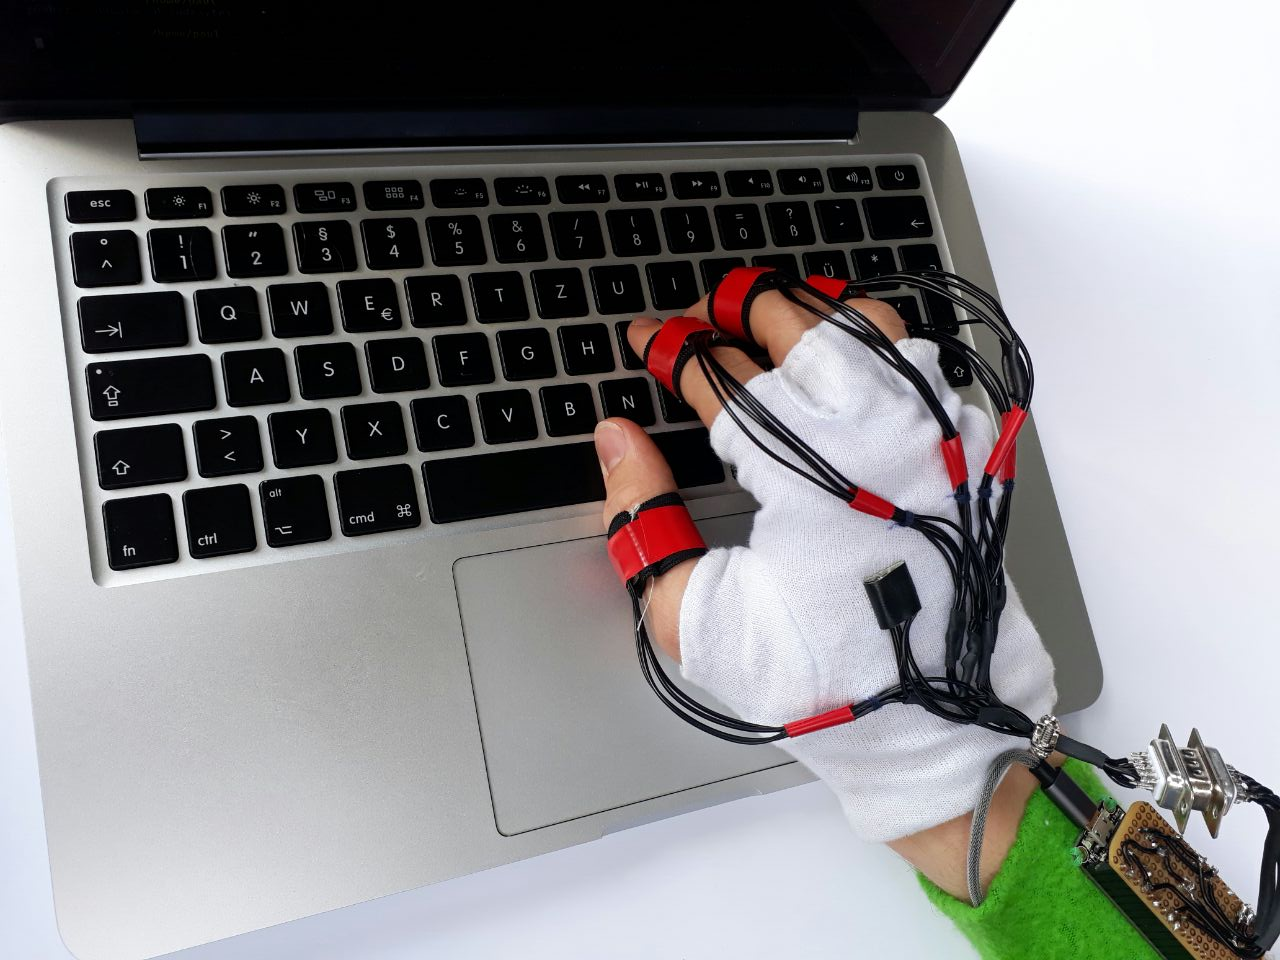
\includegraphics[width=0.8\textwidth]{../common/images/glove_laptop}}
    \caption[Der entwickelte Prototyp einer virtuellen Tastatur]{Der im Rahmen
    dieser Arbeit entwickelte Prototyp einer virtuellen Tastatur, hier gezeigt
    beim Aufzeichnen der Lerndaten. Am Handschuh sind die Sensoren (6 IMUs)
    sowie der Mikroprozessor befestigt. Auf den Mikroprozessor ist die
    Entwicklungsplatine aufgesteckt, welche Verkabelung der Sensoren
    ermöglicht.}
    \figlabel{glove_laptop}
\end{figure}

Die Entwicklung und Konfiguration des Lernalgorithmus sowie die Experimente zum
Erlernen eines Modells behandelt Carolin Konietzny in ihrer Arbeit \citep{caro}.

Die Bewertung der einzelnen Leistungen findet sich selbstverständlich in beiden
Arbeiten wieder, ebenso die Einschätzung des Gesamterfolgs unseres Projekts.

\section{Abgrenzung} \seclabel{vereinfachungen}

Im Rahmen der Bachelorarbeit schränken wir unsere Arbeiten auf einen Teilumfang
der im \secref{vision} genannten Vision ein, und sehen unser Ziel primär in der
Machbarkeitsanalyse. Wir erwarten nicht, ein fertiges Produkt zu entwickeln,
mit welchem man mühelos und einwandfrei tippen kann -- der Umfang wäre zu groß.
Daher haben wir an einigen Stellen starke Vereinfachung gewählt, um möglichst
vielen Problemen vorerst aus dem Weg zu gehen. Hierzu zählen unter anderem:

\begin{itemize}
    \item Wir konzentrieren uns auf die Durchführung mit nur einer einzelnen
        Testperson. Unsere hergestellte Hardware sowie das gelernte Modell
        müssen nicht für andere Personen anwendbar sein.
    \item Die gewählte Testperson kann blind, aus dem Muskelgedächtnis,
        unter Verwendung (fast) aller Finger tippen. Eine Tippweise, bei der
        einzelne Tasten erst gesucht oder nur mit den Zeigefingern gedrückt
        werden, muss unser System nicht unterstützen.
    \item Aus Kostengründen und zur Verringerung der Komplexität statten wir
        vorerst nur eine Hand mit Sensoren aus.
    \item Die hergestellte Hardware muss, da es sich um einen Prototyp
        handelt, keine realistischen Qualitätsanforderungen an ein
        gebrauchsfähiges und alltagstaugliches Produkt erfüllen. Beim Design
        sollte jedoch darauf geachtet werden, dass die Entwicklung hierzu
        grundsätzlich möglich ist.
    \item Das entwickelte Verfahren für das maschinelle Lernen ist eines
        von vielen möglichen. Wir gehen nicht davon aus, dass wir in unserer
        Arbeit die beste Möglichkeit finden. Dies wird weitere Forschung
        erfordern, deren Umfang unsere Arbeiten sprengen würde. Unser Ansatz
        soll als Anfang dienen, um die allgemeine Machbarkeit einschätzen zu
        können und eine Vergleichsbasis schaffen.
\end{itemize}

\section{Aufbau}

Der Hauptteil dieser Arbeit erstreckt sich über 5 Kapitel. In \chapref{ziele}
beschreibe ich die Anforderungen an das zu entwerfende System und begründe
deren Relevanz. \chapref{state-of-the-art} zeigt verwandte Arbeiten und
Projekte. Das tatsächliche Systemdesign mit den wichtigen Entscheidungen und
deren Begründungen wird in \chapref{systemdesign} erläutert. Im \chapref{ml}
gehe ich kurz auf die Anwendung und die verwendeten Prinzipien des maschinellen
Lernens ein, um dann in \chapref{bewertung} das entwickelte System zu bewerten
und mit den anfangs gestellten Zielen vergleichen zu können. Im Fazit
(\chapref{fazit}) fasse ich die Arbeit zusammen und gebe einen Ausblick auf
weitere mögliche Forschungsthemen.


% vim: tw=79
